\section{ALU}
Vi har vores 4-bit ALU ved først at implementere tre delkomponenter, som
derefter sættes sammen:
\begin{itemize}
\item 1-bit adder
\item 1-bit ALU
\item 1-bit ALU til den sidste bit, som opdager overflow samt finder ud af om
resultatet er negativt.
\end{itemize}

\subsection{1-bit adder}
Vores 1-bit adder var triviel at implementere. Den tager imod tre 1-bit input, lægger
dem sammen og giver resultaterne i form af to bits. Ud fra konteksten forstås
den ene af vores input som den indgående mente, ligesom den mest betydende bit i outputet
også forstås som den udgående mente. Dette er dog ikke relevant for
implementation. \\
\\
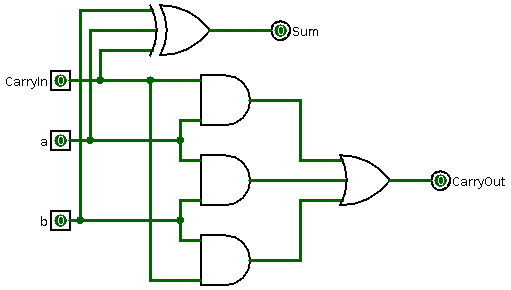
\includegraphics{Billeder/1bit-adder.png}

\subsection{1-bit ALU}
Vores 1-bit ALU tager imod fem forskellige typer input:
\begin{itemize}
\item De to tal, som der laver operationer kaldet {\tt a} og {\tt b}.
\item Information om hvorvidt {\tt a} og {\tt b} skal negeres før de bruges.
\item Den indgående mente.
\item Information om resultatet af en ``mindre end''-operation som ikke
kan udregnes ud fra en enkelt bit.
\item En 2-bits beskrivelse af hvilken operation der skal udføres på {\tt a} og
{\tt b}.
\end{itemize}

ALU'en kan som udgangspunkt udføre 4 operationer: plus, AND, OR og så kan den
bruge det eksterne resultat af en ``mindre end''-operation. Der er lavet
kredsløb til beregning af alle resultaterne og hvilket resultat der bruges
udvælges af en MUX. Desuden er der et output til den udgående mente som bruges
til den næste 1-bit ALU. \\
\\
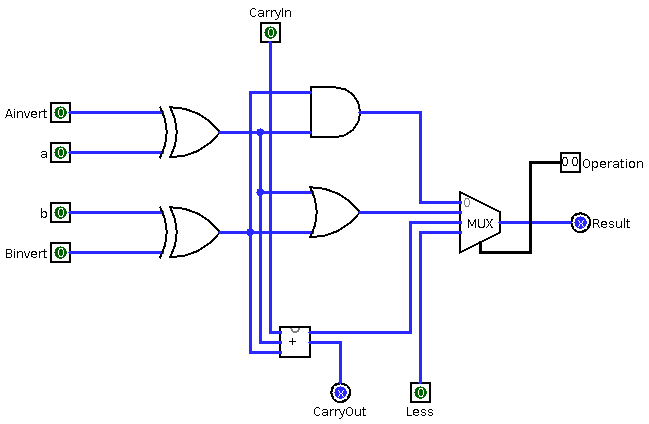
\includegraphics[angle=90]{Billeder/1bit-ALU.png}

\subsection{1-bit ALU til den sidste bit}
Den sidste 1-bit ALU er som udgangspunkt konstrueret på præcis som den
almindelige 1-bit ALU. Dog er der den forskel at der også er output pins til
overflow samt til at afgøre hvorvidt resultatet er negativt. Overflow beregnes
ved $CarryIn XOR CarryOut$.

Resultatet er desuden negativt netop når det der ikke er overflow og udregnede
resultat er negative (den sidste bit er 1) eller når der {\emph er} overflow og
der udregnedes resultat er positivt. Med andre ord $Overflow XOR Result$. \\
\\
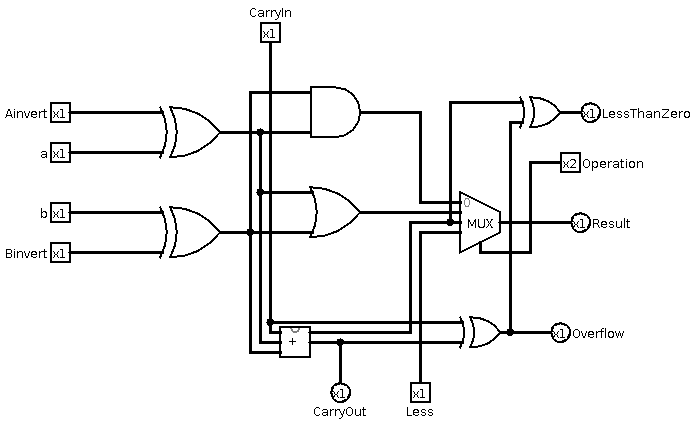
\includegraphics[angle=90]{Billeder/1bit-ALU-last.png}

\subsection{4-bit ALU}
Ud fra 1-bit ALU'erne er det trivielt at implementere en 4-bit ALU -- bare sæt
dem efter hinanden. Bitsene i ``ALU operation'' beskriver hvorvidt {\tt a} skal
negeres, hvorvidt {\tt b} skal negeres, og derefter 2 bits der beskriver hvilken
operation der er tale om. I tilfælde af at {\tt b} negeres sættes den første
mente også til 1, idet dette er en nem måde at implementere {\tt
sub}-operationen på. \\
\\
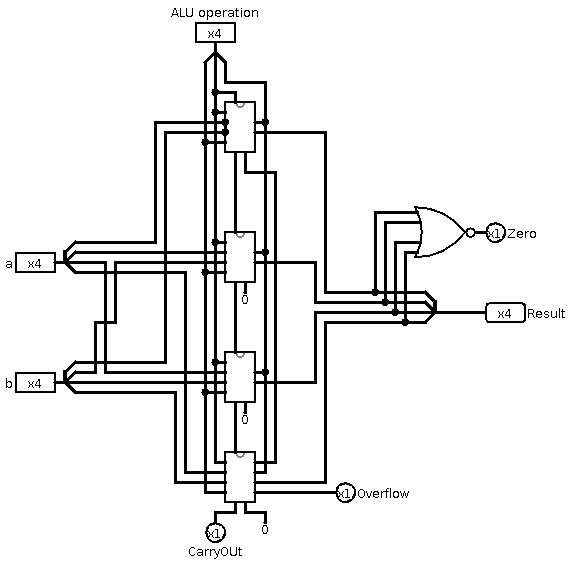
\includegraphics{Billeder/4bit-ALU.png}
